\documentclass{bmvc2k}

%% Enter your paper number here for the review copy
% \bmvcreviewcopy{??}

% \usepackage[brazilian]{babel}
\usepackage[utf8]{inputenc}
\usepackage{float}

\title{Project 2 - Fisherwalks: Statistical gait recognition}

% Enter the paper's authors in order
% \addauthor{Name}{email/homepage}{INSTITUTION_CODE}
\addauthor{Amélia O. F. da S.}{190037971@unb.br}{1}

% Enter the institutions
% \addinstitution{Name\\Address}
\addinstitution{
  Departamento de Ci\^encia da Comptuta\c{c}\~ao\\
  Universidade de Bras\'{\i}lia\\
  Campus Darcy Ribeiro, Asa Norte\\
  Bras\'{\i}lia-DF, CEP 70910-900, Brazil  
}

\runninghead{Oliveira F. da S., Amélia}{Computer Vision Assignment -- \today}

% Any macro definitions you would like to include
% These are not defined in the style file, because they don't begin
% with \bmva, so they might conflict with the user's own macros.
% The \bmvaOneDot macro adds a full stop unless there is one in the
% text already.
\def\eg{\emph{e.g}\bmvaOneDot}
\def\Eg{\emph{E.g}\bmvaOneDot}
\def\etal{\emph{et al}\bmvaOneDot}

%-------------------------------------------------------------------------
% Document starts here
\begin{document}

\maketitle

\begin{abstract}

   Fisher's Linear Discriminant Analysis is a commonly used tool for dimensionality reduction and linear classification. This paper proposes a new application of Fisher's Discriminant to distinguish between subjects using gait features, facilitating subject identification when other methods such as facial identification are unfeasible.

\end{abstract}

\section{Introduction}

\begin{center}

   When two or more populations have been measured in several characters \textit{$x_1$, ... , $x_8$}, special interest attaches to certain linear functions of the measurements by which the populations are best discriminated.

   \begin{flushright}
      \textit{
         Ronald A. Fisher - "The Statistical Utilization Of Multiple Measurements"\\
         1936
      }
   \end{flushright}
\end{center}

Fisher’s Linear Discriminant Analysis (henceforth “LDA”) has been utilised in a multitude of fields across its long history to classify and differentiate populations, from medical data analysis to face recognition (where it is widely known as the Fisherfaces method).

LDA fundamentally provides us with a projection in which dispersion within the classes is minimised and class separation is maximised\cite{fisher}. This allows a multi-variable problem to be treated as a single-variable problem or a simpler multi-variable problem by projecting the data onto axes which describe a more marked distinction between the classes\cite{dimred}\cite{statanalysis}.

This paper proposes an application for LDA as a way to make subject recognition simpler and applicable on a wider range of contexts through identification by gait analysis. The proposed method allows for identification in situations where facial recognition and other methods might fail or where features might be intentionally concealed.

\section{Methodology}

\subsection{Pose analysis}

The \textit{OpenPose}\cite{op1}\cite{op2}\cite{op3}\cite{op4} system was used to provide a rough estimate of the subjects' 3D poses (precise positioning would require multiple views or depth cameras) at four different key points in their walk cycle: the points of maximum and minimum leg extension for both left and right paces.

\begin{figure}[H]
   \begin{center}
      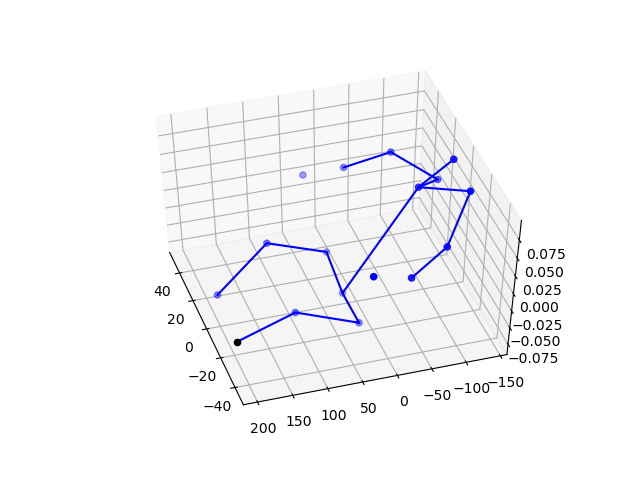
\includegraphics[width=5cm]{figures/OPOut.png}
      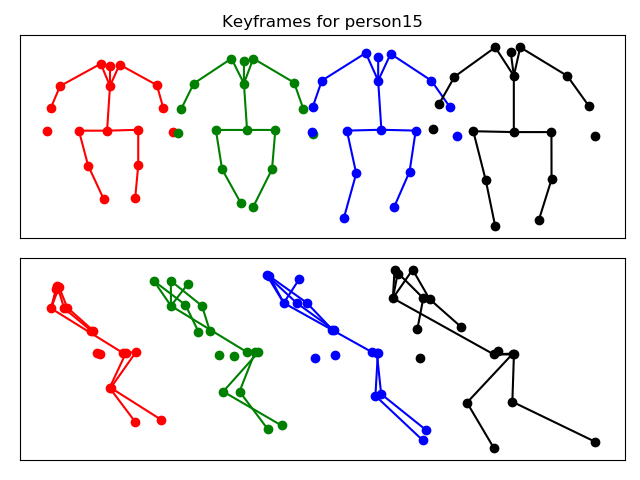
\includegraphics[width=5cm]{figures/walkdata.png}\\
   \end{center}
   \caption{Sample output for OpenPose and a full collected sample}
\end{figure}

From each pose estimate, eight angle measurements were made:

\begin{itemize}
   \item Left and right torso-arm angles ("armpit")
   \item Left and right elbow angles
   \item Left and right hip-thigh angles
   \item Left and right knee angles
\end{itemize}

That provides eight scale-independent features for each point in time, resulting in 32 angle dimensions. The standard deviation  for each key angle was also calculated and added as a feature for a description of their variation along the walk cycle. This set of features describes a 40-dimensional sample vector.

\subsection{Linear Discriminant Analysis}

For any given set of samples for two or more classes, there exists a projection axis (which can also be seen as a function of the original axes) on which the projections of the classes will show maximum class mean separation and minimal spread within the classes\cite{fisher}. Assuming the classes are unimodal and follow a Gaussian distribution, we can calculate that axis using Fisher's Linear Discriminant.

\begin{figure}[H]
   \begin{center}
      \begin{tabular}{p{5cm} p{5cm}}
         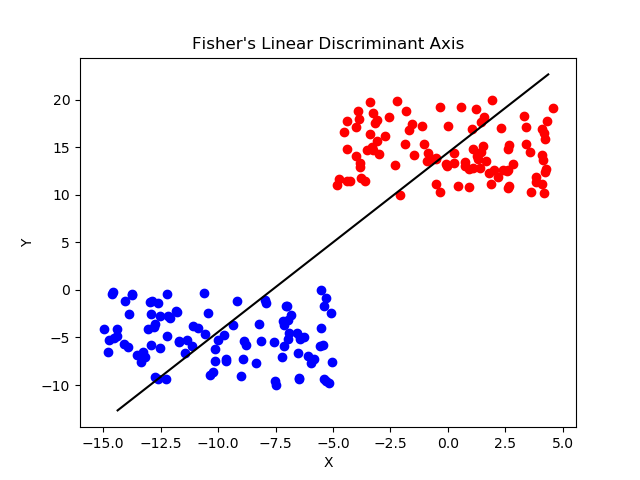
\includegraphics[width=5cm]{figures/fisher2classes.png}&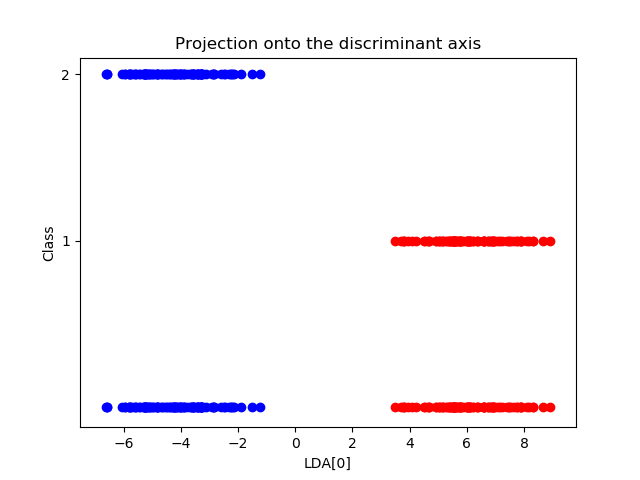
\includegraphics[width=5cm]{figures/fisherProjection2classes.png}\\
         Scatterplot of two classes in 2D and the optimal discriminant axis&Projection along the described axis evidencing the separation
      \end{tabular}
   \end{center}
   \caption{A 2D visualisation of Fisher's Linear Discriminant}
\end{figure}

Fisher's linear discriminant can be calculated using \textit{Scatter Matrices}, which approximate the covariance between variables in a set\cite{fisherUt}. Since the final goal is to maximise the scatter \textit{between} classes and minimise the scatter \textit{within} the classes, two scatter matrices will be needed:
\begin{equation}\label{scatter}
   S_B := N_{classes}*Scatter(class\ means),\  
   S_W := \sum^{Classes}Scatter(samples_{class})
\end{equation}
With
\begin{equation}
   Scatter(X) := \sum_{i=0}^{i=N_X} (vector_i-Mean(X))(vector_i-Mean(X))^T
\end{equation}

The simultaneous maximisation of scatter "between" classes and minimisation of scatter "within" classes can be represented as the maximisation of a ratio between both (see Appendix 1.1 \cite{appendix} for a thorough description of that maximisation process). The vector $W$ that maximises that ratio will then be defined as:

\begin{equation}\label{eigen}
   W :=  argmax_W(|W^T\ S_B\ S_W^{-1}\ W|)
\end{equation}

Solving that maximisation problem is equivalent\cite{face} to solving an eigenvector problem for that resulting matrix, allowing us to easily compute the optimal vectors.

\subsection{One-against-all projections}

LDA allows us to calculate the optimal $N-1$ axes to separate $N$ classes, but for multi-class classification problems we can also adopt a more intuitive (and often more effective) "One-against-all" approach, also known as "Binary Relevance"\cite{binary}. That approach consists in focusing on indidvidually separating classes from all others instead of generating a general classifier. For that, multiple discriminant analyses were used to find $N$ axes that individually separate each class from the others, greatly simplifying classification.

\begin{figure}[H]
   \begin{center}
      \begin{tabular}{c c c}
         \multicolumn{3}{c}{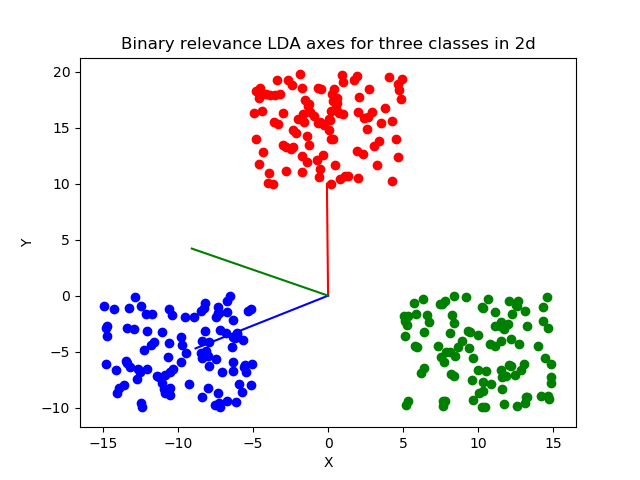
\includegraphics[width=4.5cm]{figures/binaryRelevance3classes.png}
         }\\
         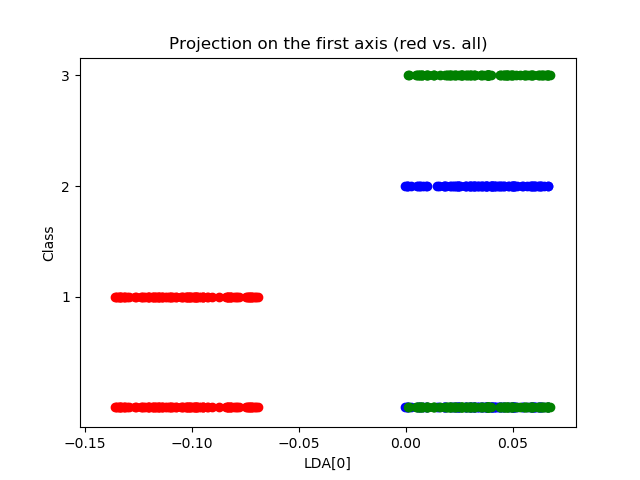
\includegraphics[width=3cm]{figures/projectionRedAll.png}&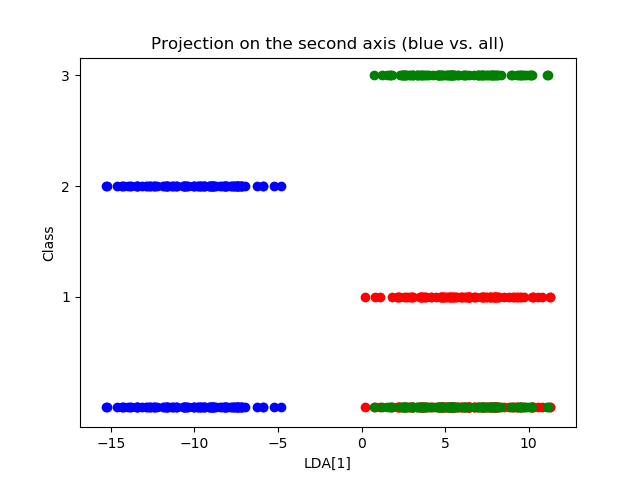
\includegraphics[width=3cm]{figures/projectionBlueAll.png}&
         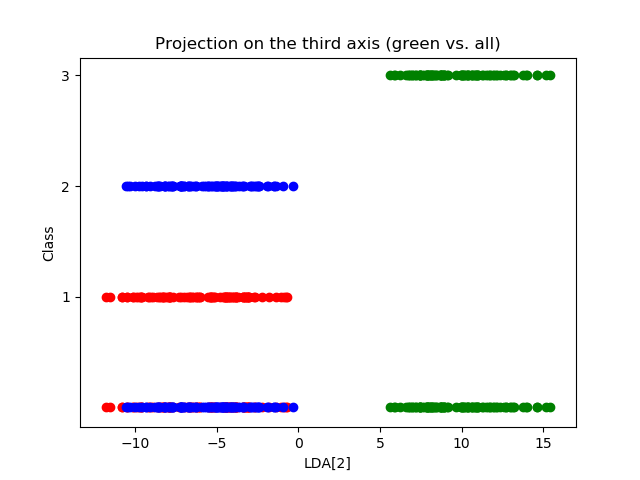
\includegraphics[width=3cm]{figures/projectionGreenAll.png}\\
         Red axis&Blue axis&Green axis
      \end{tabular}
   \end{center}
   \caption{2D One-against-all discriminant axes for 3 classes}
\end{figure}

\begin{figure}[H]
   \begin{center}
      \begin{tabular}{p{5cm} p{5cm}}
         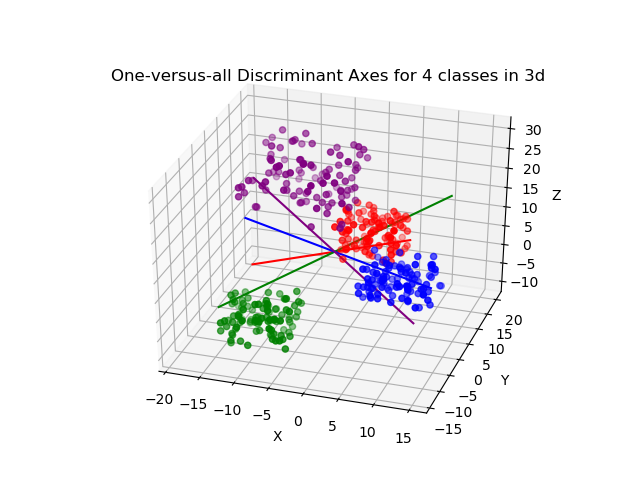
\includegraphics[width=5cm]{figures/3ddiscriminantAxes.png}&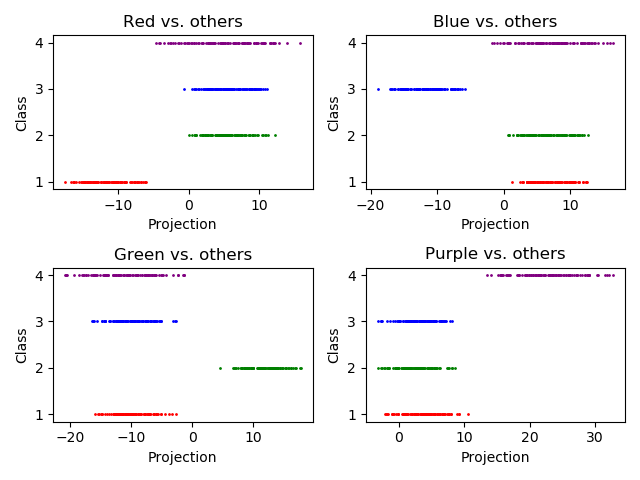
\includegraphics[width=5cm]{figures/3dProjections.png}\\
         Scatterplot of four classes in 3D and the "One-versus-all" axes&Projections along the resulting axes evidencing the separation between each class and the others
      \end{tabular}
   \end{center}
   \caption{3D One-against-all discriminant axes for 4 classes}
\end{figure}

\subsection{Principal Component Analysis}

Calculating the scatter matrices (eq. \ref{scatter}) yields a problem when dealing with many dimensions: those matrices will be singular when the number of dimensions is greater than the number of samples used, turning the inverse matrix calculation impossible\cite{singular}.

A solution for this problem is to first apply other dimensionality reduction methods to the data so the number of dimensions matches the number of samples\cite{face}. Here, \textit{Principal Component Analysis} was used to extract the $min(N_{class})$ projection axes along which the data has the most variance.

\begin{figure}[H]
   \begin{center}
         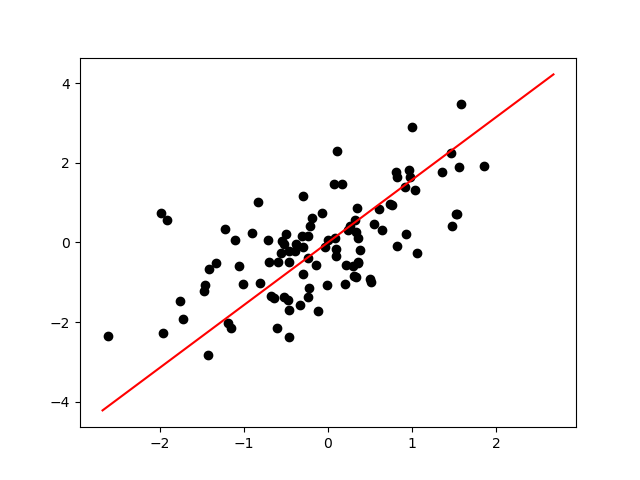
\includegraphics[width=5cm]{figures/PCA.png}
   \end{center}
   \caption{A 2D visualisation of the the first axis generated by PCA}
\end{figure}

The Principal Component Analysis problem is mathematically equivalent to the "least squares" problem or Eignevector decomposition and can be performed as following:

Given a set $S$ of vectors (our full dataset)
\begin{equation}
   W := argmin_W(|Scatter(S)|)
\end{equation}
Which is also an eigenvector problem (see eq. \ref{eigen} and Appendix 1.1 \cite{appendix}).

\section{Results}

\subsection{Implementation description}

The statistical methods above were implemented using the Numpy\cite{numpy} scientific computing package in Python.

Due to processing power limitations, the key images for each sample had to be manually separated and then processed through the proposed pipeline. This limited the test sample size to four classes of six 4-image samples each, totalling 96 images.

Provided with the extracted sample vectors, the program generates a single projection matrix $P$ that combines the PCA and LDA projections as following:

Let $D$ be a data matrix containing $n$ 40-dimensional column vectors of $c$ classes and a minimum number $m$ of samples per class.

Let $R$ be our resulting projected data matrix.
\begin{equation}
   \begin{split}
      R_{cXn} := LDA_{cXm} \ PCA_{mX40} \ D_{40Xn}\\
      R_{cXn} = (LDA_{cXm}\ PCA_{mX40})\ D_{40Xn}\\
      R_{cXn} = P_{cX40}\ D_{40Xn}
   \end{split}
\end{equation}

For ease of implementation, line vector notation was used in the code instead of the standard column vector notation, meaning in practice calculations will be done in the reverse order (right to left, with all matrices transposed).

\subsection{Feature importances}

It is possible to estimate the importance of each measured feature by measuring its final weight on the projection\cite{statanalysis}.

\begin{figure}[H]
   \begin{center}
      \begin{tabular}{c c}
         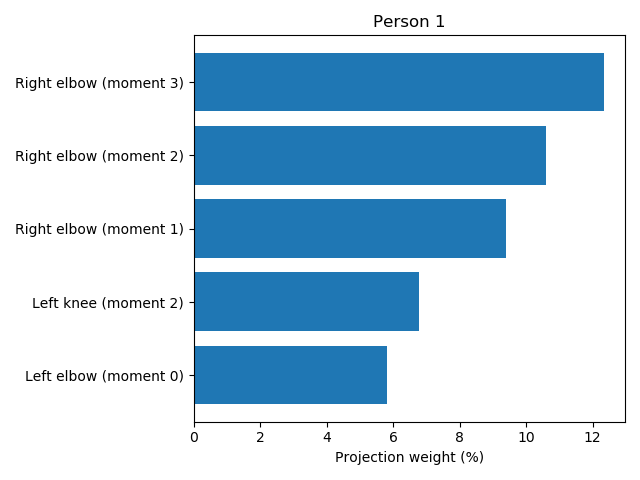
\includegraphics[width=6cm]{figures/person1Imp.png}&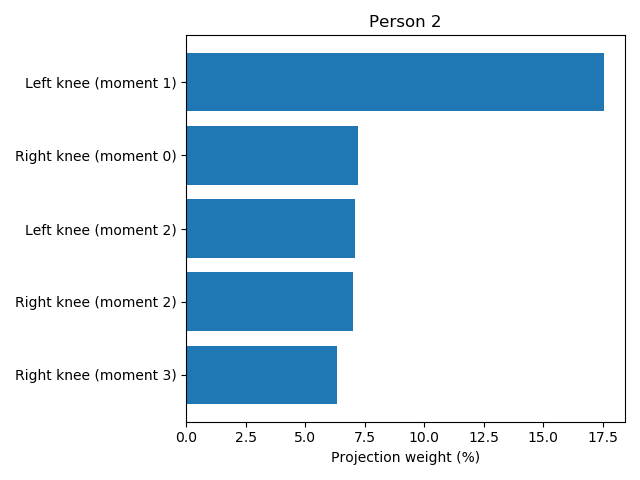
\includegraphics[width=6cm]{figures/person2Imp.png}\\
         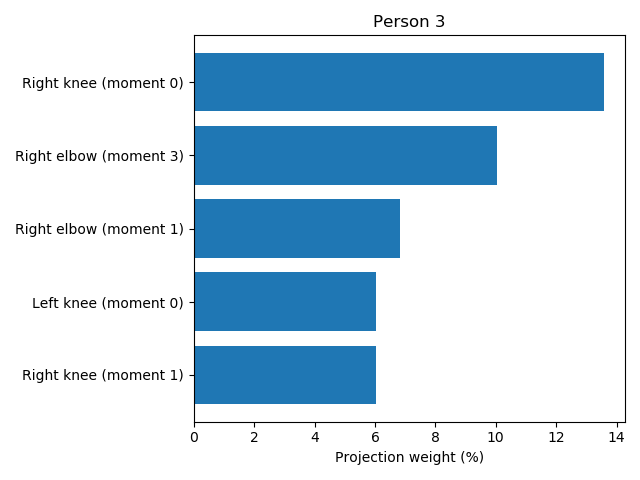
\includegraphics[width=6cm]{figures/person3Imp.png}&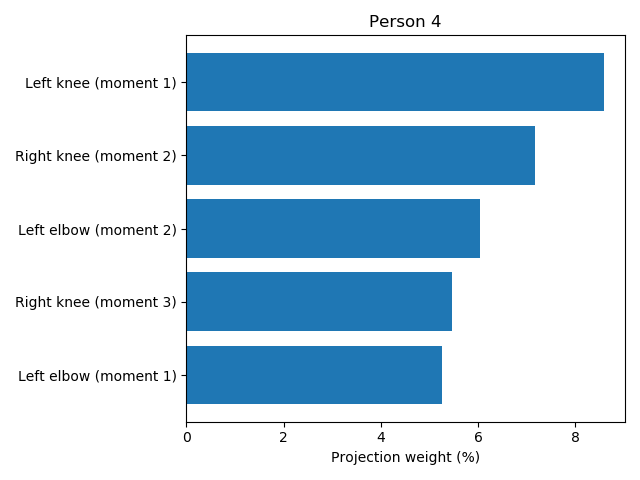
\includegraphics[width=6cm]{figures/person4Imp.png}
      \end{tabular}
   \end{center}
   \caption{Feature importances for the four subjects}
\end{figure}

Those results can be interpreted as the main discriminating characteristics for each sub-ject\cite{statanalysis}. Those characteristics reflect visually perceptible differences between the subjects (See Appendix 1.4 \cite{appendix}).

\subsection{Classification tests}

Due to the small number of samples, the tests were limited to evaluating how well the projections describe the class space instead of the typical "training" vs. "testing" sets. 
The following methods were used for that purpose:

\subsubsection{Nearest Mean}

Given the projection axes, each sample's label was assigned according to the closest class mean on that projection (Euclidean distance). All samples were assigned the correct class.

The LDA projection can significantly improve nearest mean classification on situations where axes are imbalanced scale-wise\cite{statanalysis} (see Appendix 1.2 \cite{appendix}).

\begin{figure}[H]
   \begin{center}
      \label{m1}
      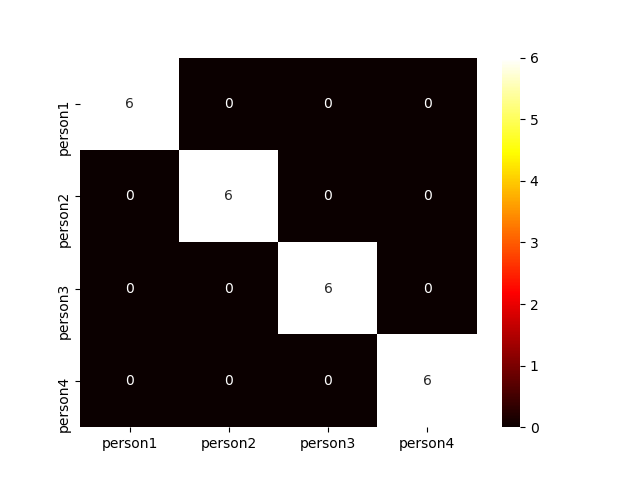
\includegraphics[width=6cm]{figures/ConfusionMatrixNearestMean.png}
   \end{center}
   \caption{Nearest Mean Confusion Matrix}
\end{figure}

\subsubsection{Thresholding on individual dimensions}

An advantage of using Binary Relevance classification is the possibility of establishing a single threshold ($\frac{\mu_A+\mu_b}{2}$) on each axis for deciding whether a sample belongs to a class (linear classification)\cite{binary}. This allows for quickly determining whether individuals belong to a certain class without the need to compare them with other references.

\begin{figure}[H]
   \begin{center}
      \label{m2}
      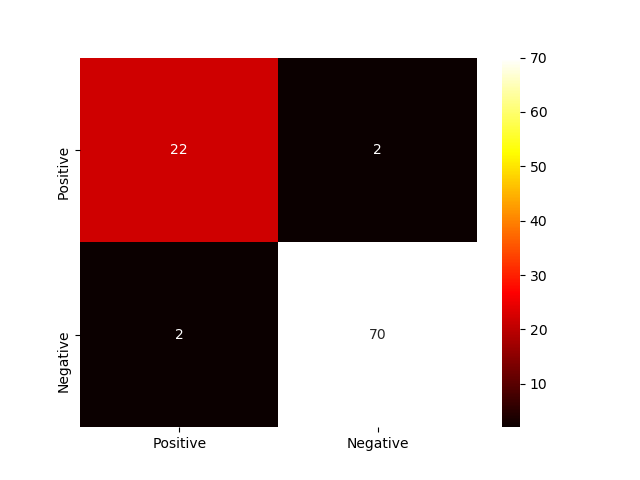
\includegraphics[width=6cm]{figures/ConfusionMatrixSingleAxis.png}
   \end{center}
   \caption{Single-Axis thresholding Confusion Matrix}
\end{figure}

This method yielded 4 misclassifications out of 96 samples in total (see Appendix 1.3 \cite{appendix} for more information on what caused those misclassifications).

\section{Conclusion}

Although the number of samples was limited by the processing power available, the results obtained seem to prove the method's usefulness in practical applications. The resulting projections not only accurately separated the classes but also matched visually perceptible and intuitive patterns (see Appendix 1.1 \cite{appendix}).

The proposed method would benefit from further research, especially on automatically extracting the key images used in processing (through faster pose extraction methods) and testing the resulting performance on larger datasets.

\bibliography{refs}
\end{document}
